\documentclass[12pt,a4paper]{article}

\usepackage[margin=2.5cm]{geometry}
\usepackage{amsmath,amssymb}
\usepackage{graphicx}
\usepackage{booktabs}
\usepackage{longtable}
\usepackage{array}
\usepackage{float}
\usepackage{xcolor}
\usepackage{hyperref}
\usepackage{enumitem}
\usepackage{caption}
\usepackage{subcaption}

\hypersetup{
  colorlinks=true,
  linkcolor=blue,
  citecolor=blue,
  urlcolor=blue
}

\newcommand{\code}[1]{\texttt{#1}}
\newcommand{\fitness}{\operatorname{fit}}
\newcommand{\rank}{\operatorname{rank}}

\title{\textbf{Mid-Term Report for Master's Thesis}\\[0.5em]
Research on the Design of Evolutionary Algorithms for Multimodal Optimization}
\author{
School of Computer Science and Technology\\
Harbin Institute of Technology, Shenzhen\\[0.5em]
Graduate Student: IRSHAD HAMZA\\
Supervisor: Professor Wenjian Luo
}
\date{June 2026}

\begin{document}
\maketitle
\thispagestyle{empty}

\begin{center}
\vfill
Shenzhen Department of Academic Affairs
\end{center}
\newpage

\tableofcontents
\newpage

\section{Research Background and Objectives}

The original thesis proposal identified a gap between two related research lines:
multimodal optimization (MMO), which searches for multiple high-quality optima in a
single landscape, and multiparty multiobjective optimization (MPMO), which models
multiple decision-makers but usually emphasizes one common compromise set. Many
real decision-making problems require both capabilities simultaneously. In unmanned
aerial vehicle path planning, for example, an efficiency-oriented party may prefer short
flight time and low energy consumption, while a safety-oriented party may emphasize
risk reduction. A single compromise is often not enough; several spatially distinct
solutions may be equally valuable because they provide different implementation
choices and robustness against uncertainty.

This project therefore studies \emph{Multiparty Multimodal Optimization} (MPMMO).
An MPMMO problem is defined on a shared decision space $\Omega \subseteq \mathbb{R}^D$
and a set of party objectives
\begin{equation}
  F(x)=\{F_1(x),F_2(x),\ldots,F_M(x)\}, \quad x \in \Omega ,
\end{equation}
where each $F_i$ represents the preference landscape of one decision-maker. The goal is
not only to obtain high values for all parties, but also to discover multiple decision-space
regions that are jointly acceptable. In this report the current implementation focuses on
the two-party case, so $F(x)=(F_0(x),F_1(x))$.

The mid-term work follows the objectives in the proposal: first, to construct a scalable
and tunable MPMMO benchmark suite based on the OFEC FreePeak framework; second, to
design an evolutionary algorithm that maintains party-wise multimodal diversity while
coordinating common optima across parties; third, to validate the implementation against
multimodal multiobjective algorithms in PlatEMO.

\section{Literature Review}

\subsection{Multimodal Optimization and Niching}

Multimodal optimization algorithms attempt to locate more than one optimum in the
decision space. Classical niching strategies, including fitness sharing, clearing, crowding,
speciation, and clustering-based methods, reduce the tendency of a population to collapse
into one basin. Nearest-better clustering (NBC) and nearest-better networks (NBN) are
especially useful because they infer basin structure directly from sampled individuals.
Each solution is connected to the nearest solution with better fitness, and long edges
often indicate boundaries between basins.

\subsection{Multiparty Multiobjective Optimization}

MPMO models optimization with several decision-makers, each holding different
preferences. Earlier studies such as OptMPNDS and related multiparty nondominated
sorting methods focus on representing common Pareto optimality under distributed
objectives. These methods are important for multi-stakeholder optimization, but they do
not explicitly preserve multiple decision-space optima that lead to similar objective
quality.

\subsection{Research Gap}

The gap is that MMO and MPMO have mostly been developed separately. MMO methods
usually assume one objective or one standard multiobjective problem, while MPMO
methods usually focus on one compromise set. MPMMO requires a benchmark and an
algorithmic framework that can represent shared optima, party-private optima, conflicting
local basins, and heterogeneous landscape difficulty at the same time.

\section{Work Completed}

\subsection{Benchmark Problem Design}

\subsubsection{FreePeak-Based Multiparty Construction}

The new benchmark suite is implemented on top of OFEC FreePeak. The original FreePeak
framework partitions the normalized decision space $[0,1]^D$ by a k-d tree and assigns
one peak function to each leaf subspace. This makes the number of subspaces, peak
locations, heights, attraction-domain sizes, and transformations independently
controllable.

The multiparty extension gives each party its own k-d tree:
\begin{equation}
  F_i(x) = P_i(x;\mathcal{T}_i,\mathcal{O}^{\mathrm{shared}},
  \mathcal{O}^{\mathrm{private}}_i),
\end{equation}
where $\mathcal{T}_i$ is the party-specific k-d tree, $\mathcal{O}^{\mathrm{shared}}$
contains optima placed at identical decision-space positions for all parties, and
$\mathcal{O}^{\mathrm{private}}_i$ contains optima preferred only by party $i$.
The consensus fitness used by the algorithm and metrics is
\begin{equation}
  C(x)=\min(F_0(x),F_1(x)).
\end{equation}
Therefore, a point is a true common optimum only if it is good for both parties.

Different parties are deliberately assigned different k-d tree divisions. As a result, the
same point may belong to different leaf subspaces under different party objectives. This
is important because it creates asymmetric attraction domains and party-dependent local
conflicts. Shared optima are generated by selecting overlapping regions across parties and
placing identical peak centers in those regions; private optima are sampled randomly in
the remaining party-specific leaf spaces.

\subsubsection{Objective Mapping and Distance Model}

The implementation uses the \code{FlatBorder} distance model and a \code{map\_objective}
transformation so that each subproblem objective is mapped to a controlled fitness range.
The mapping keeps objective values comparable across heterogeneous one-peak functions.
For visualization and algorithmic evaluation, party fitness values are normalized to a
maximization scale, with high-quality shared peaks close to 90.

\subsubsection{Landscape Transformations}

To make the suite challenging and visually distinct, each leaf subproblem can use a
different transformed one-peak function. The current implementation includes:
\begin{itemize}[leftmargin=2em]
  \item rotated basins, where the local coordinate system is rotated before evaluation;
  \item ill-conditioned basins, where attraction domains are elongated by anisotropic scaling;
  \item rugged basins, where local oscillations disturb the smooth peak shape;
  \item deceptive basins, where a broad suboptimal attraction domain competes with a
        smaller true optimum;
  \item hierarchical basins, where broad coarse structures and sharp local peaks coexist;
  \item disconnected or conflict landscapes, where party optima are separated or only
        partially aligned.
\end{itemize}
These transformations are applied through inverse or center-preserving mappings so that
the optimum position remains fixed after transformation. This is essential: the same
shared optimum must remain at the same decision-space position even when party
landscapes have different geometry.

\subsubsection{Twelve Test Problems}

The suite now contains twelve two-party base problems. The first eight emphasize one
dominant characteristic, while the last four contain more mixed structures and a larger
number of shared optima. All problems can be extended to $D=2,3,5,10$.

\begin{longtable}{p{0.12\linewidth}p{0.26\linewidth}p{0.52\linewidth}}
\caption{FreePeaks-MPMMO benchmark suites.}\\
\toprule
Suite & Name & Main characteristics \\
\midrule
\endfirsthead
\toprule
Suite & Name & Main characteristics \\
\midrule
\endhead
P1 & balanced & Several visible shared peaks with comparable basin sizes; used as the basic sanity-check problem.\\
P2 & unequal basins & Strongly unequal attraction domains; large and small basins coexist.\\
P3 & local conflict & Party objectives contain nearby but non-identical local optima, creating local disagreement.\\
P4 & rugged & Peak surfaces contain rugged perturbations and visible local irregularities.\\
P5 & rotated & Basins are rotated and anisotropic but wider than the earlier thin-line version.\\
P6 & deceptive & A large suboptimal basin is placed close to a smaller true optimum, testing whether the algorithm can escape broad attraction.\\
P7 & hierarchical & Broad hierarchical structure with embedded sharper peaks.\\
P8 & disconnected & Disconnected high-quality regions and party-dependent partitions.\\
P9 & many optima & A 20-shared-optima problem for testing multimodal coverage.\\
P10 & mixed rotated-rugged-deceptive & Mixed subspace features; different parties may use different transformations in corresponding regions.\\
P11 & mixed hierarchical-conflict & Hierarchical landscapes combined with local conflicts and party-private optima.\\
P12 & full mixed multimodal & Dense mixed-feature suite with multiple shared and private optima.\\
\bottomrule
\end{longtable}

\subsection{Visualization Protocol}

The two-dimensional version is used for direct landscape inspection. Three views are
generated for all twelve problems:
\begin{itemize}[leftmargin=2em]
  \item party-0 objective landscape $F_0(x)$;
  \item party-1 objective landscape $F_1(x)$;
  \item rank landscape obtained from the two-objective values.
\end{itemize}
The single-party plots check whether the intended feature is visible, while the rank
landscape shows the joint multiparty structure. A low-rank region represents a
nondominated or near-nondominated decision-space area under the two party objectives.

\begin{figure}[H]
  \centering
  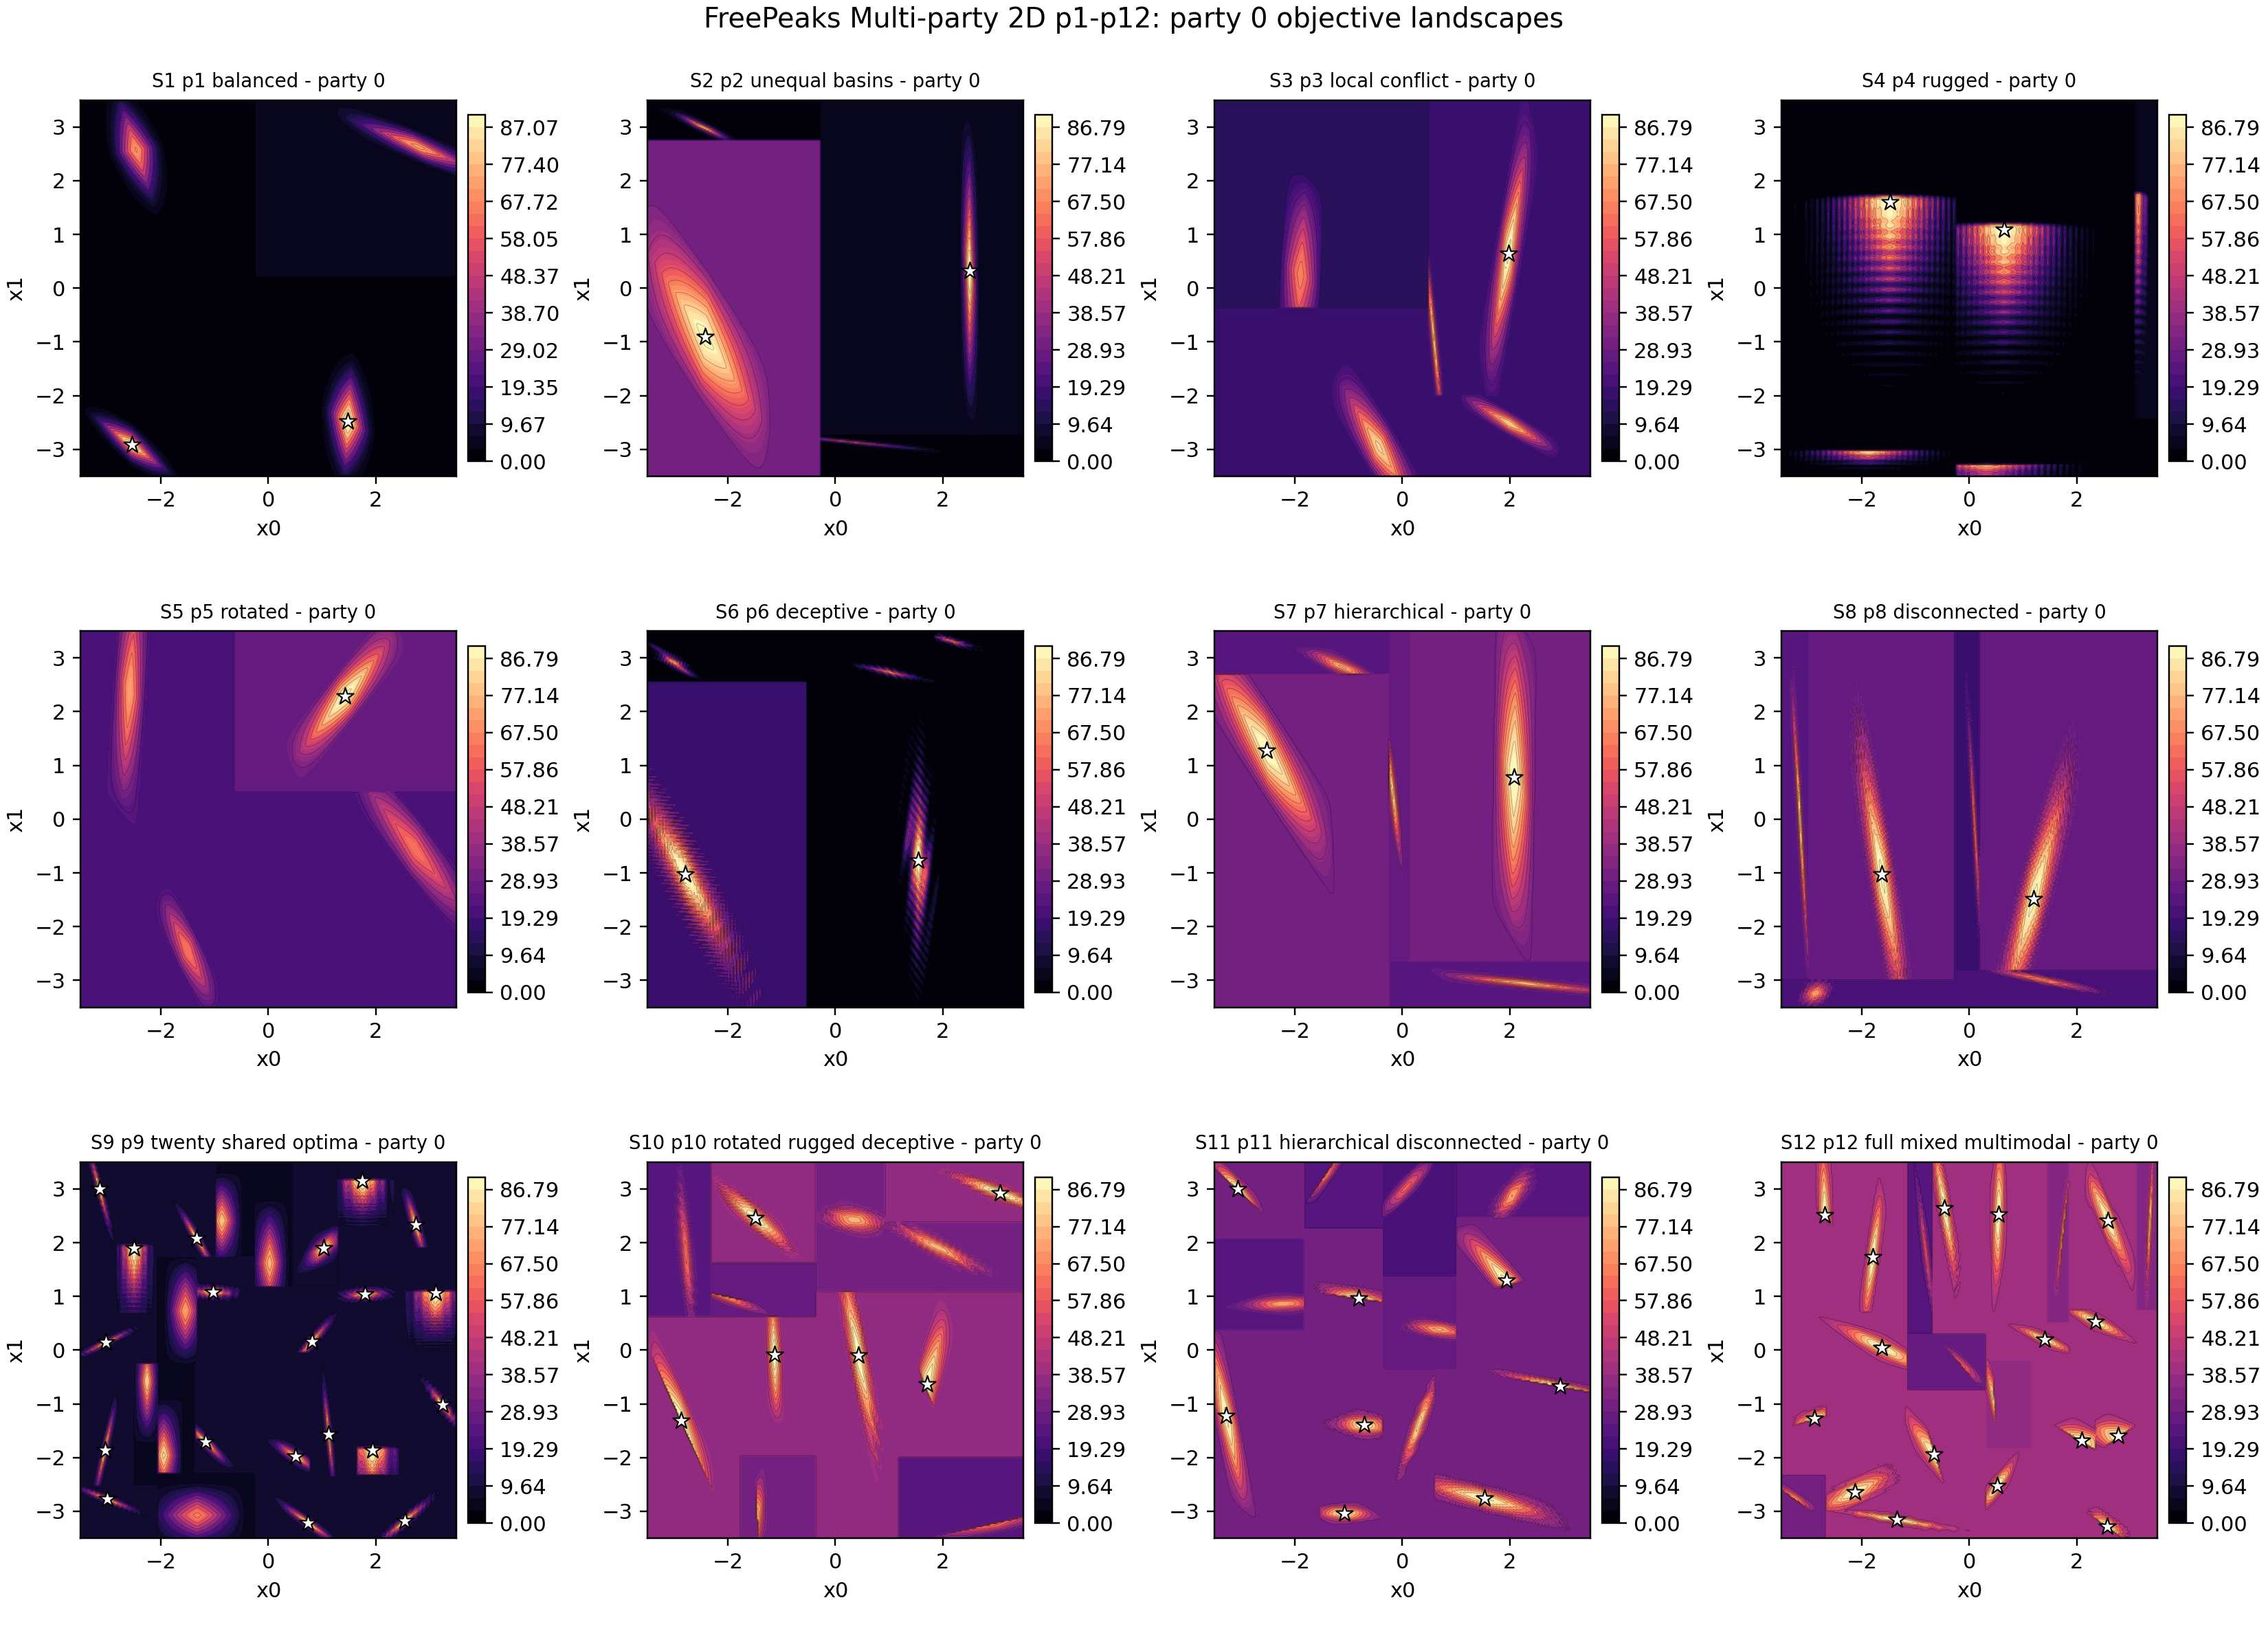
\includegraphics[width=\linewidth]{../../Visualization/figures/free_peaks_multiparty_p1_p12_party0_objective_3x4.png}
  \caption{Party-0 objective landscapes for P1--P12.}
  \label{fig:party0}
\end{figure}

\begin{figure}[H]
  \centering
  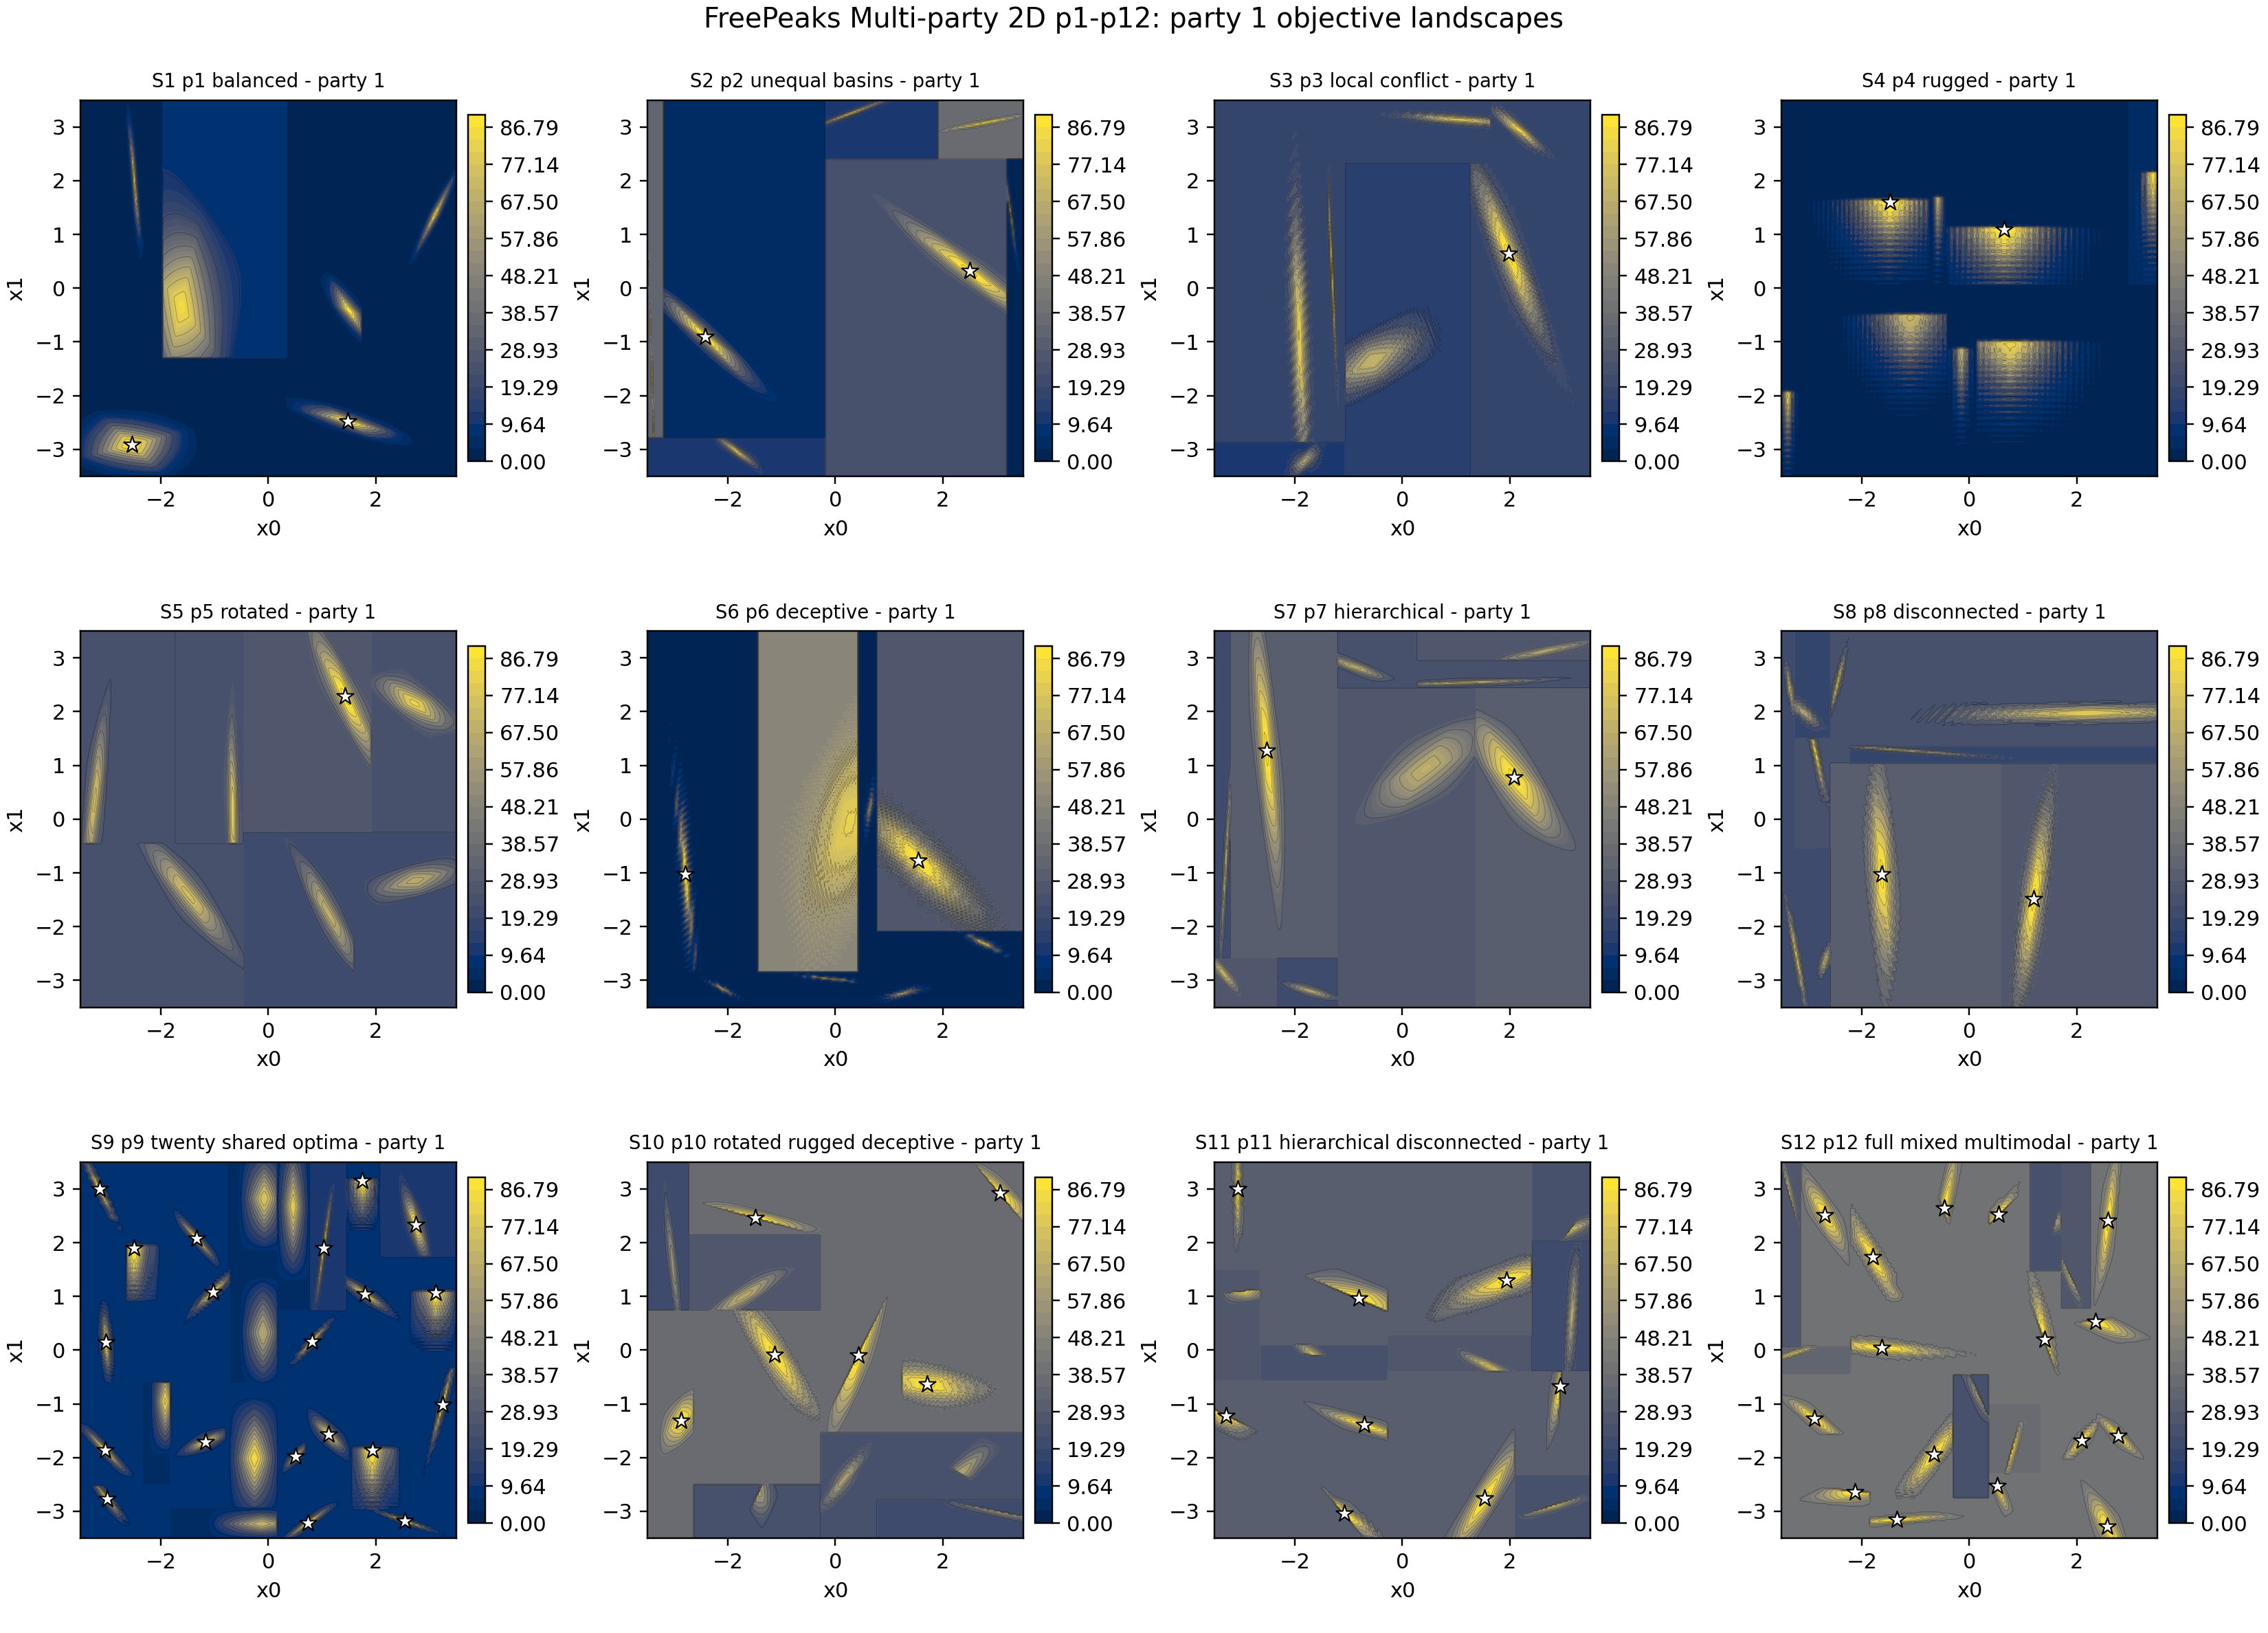
\includegraphics[width=\linewidth]{../../Visualization/figures/free_peaks_multiparty_p1_p12_party1_objective_3x4.png}
  \caption{Party-1 objective landscapes for P1--P12. Each party uses a different k-d tree and may assign different transformations to corresponding regions.}
  \label{fig:party1}
\end{figure}

\begin{figure}[H]
  \centering
  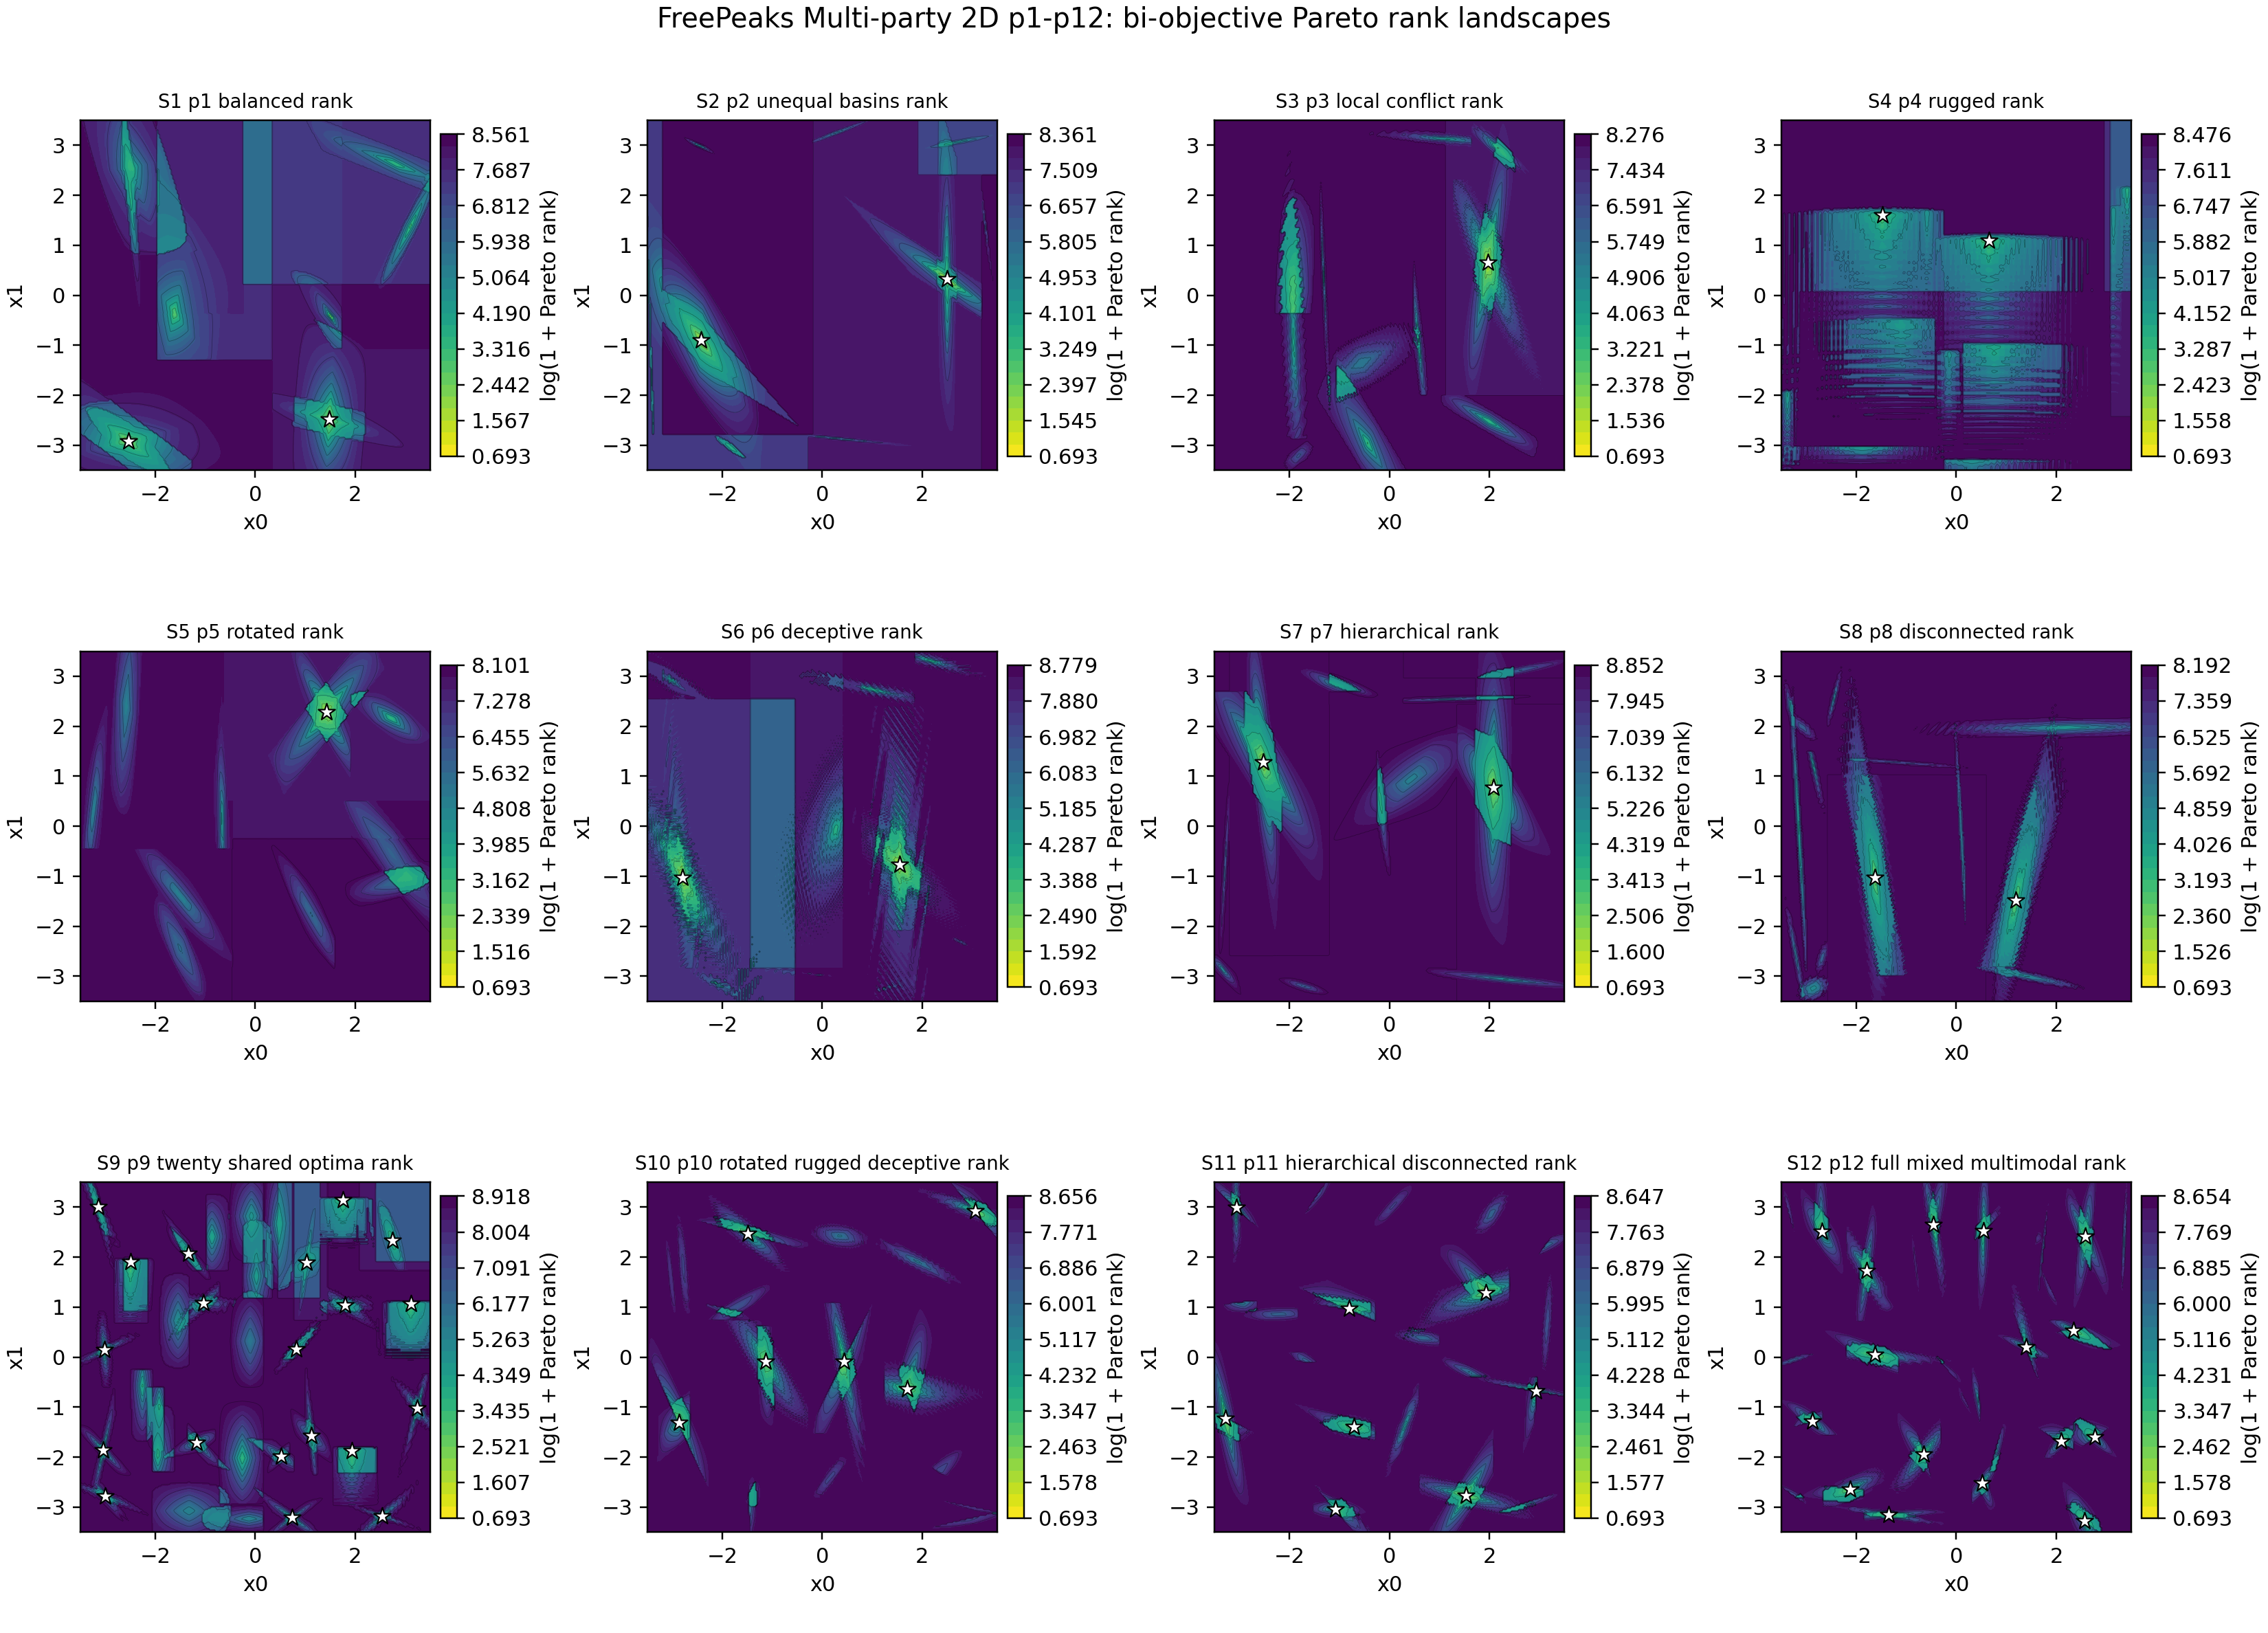
\includegraphics[width=\linewidth]{../../Visualization/figures/free_peaks_multiparty_p1_p12_rank_landscape_3x4.png}
  \caption{Two-objective rank landscapes for P1--P12.}
  \label{fig:rank}
\end{figure}

\section{Algorithm Design: Multiparty NBN-CMAES}

\subsection{Design Motivation}

The proposed algorithm follows a simple principle: each party landscape should first be
treated as a multimodal single-objective problem, and the cross-party compromise should
then be coordinated from the party-wise basins. Directly optimizing only $C(x)=\min(F_0,F_1)$
can prematurely discard useful party-specific basins, while optimizing only one party
ignores common optimality. The algorithm therefore maintains:
\begin{itemize}[leftmargin=2em]
  \item one population for each party objective;
  \item a coordination population for common optima;
  \item a full-history archive storing all evaluated individuals;
  \item a consensus archive storing diverse high-quality common solutions.
\end{itemize}

\subsection{Nearest-Better Network and NBD Clustering}

At each update, all historical evaluated individuals are stored in \code{archive\_all\_history}.
For each party, a diverse subset of the history archive is selected as the NBN working set.
Each individual is connected to the nearest individual with better party fitness. Long NBN
edges are removed according to the NBD rule, and connected components become basins or
niches. The party population is then rebuilt from these NBD clusters before local search.

This is a key change from the earlier implementation. The previous version rebuilt NBN
only from the current population, while the current version uses the accumulated history.
This makes the basin model more stable and reduces the chance of forgetting previously
found optima.

\subsection{CMA-ES Subpopulation Search and Coordination}

For each NBD cluster, the cluster-best individual is used as a local mean. The average
distance from the cluster members to the best individual determines the sampling radius.
Offspring are sampled around each basin using a lightweight CMA-ES-style Gaussian
mutation. The coordination population receives elite individuals from the party clusters
and from the consensus archive, then evolves them by differential mutation and local
Gaussian refinement.

\begin{figure}[H]
\centering
\fbox{\begin{minipage}{0.92\linewidth}
\textbf{Multiparty NBN-CMAES framework}
\begin{enumerate}[leftmargin=2em]
  \item Initialize party populations and coordination population.
  \item Evaluate all individuals and insert every evaluated individual into the full-history archive.
  \item For each party, build an NBN from the historical archive working set.
  \item Apply NBD clustering and rebuild the party population from the resulting basins.
  \item Evolve each party basin by CMA-ES-style local sampling.
  \item Update the coordination population with party elites and archive elites.
  \item Evolve the coordination population and update the consensus archive.
  \item Stop when the maximum number of function evaluations is reached.
\end{enumerate}
\end{minipage}}
\caption{Algorithm framework of the current NBN-CMAES implementation.}
\label{fig:algorithm-framework}
\end{figure}

\section{Experimental Results and Analysis}

\subsection{Experimental Settings}

The benchmark is tested on all twelve suites and four dimensions:
\[
  D \in \{2,3,5,10\}.
\]
The current report uses a practical mid-term budget of $10^5$ function evaluations for
each algorithm--problem--dimension task. The final thesis experiments will use $10^6$
function evaluations as the unified formal budget.

The proposed algorithm is compared with five PlatEMO multimodal multiobjective
algorithms: MMOPSO, MMOEABH, MMEAWI, MMEAARM, and HHCMMEA. Because PlatEMO
uses minimization and OFEC uses maximization, the wrapper problem \code{FreePeaksMPMMO}
maps objectives by $100-F_i(x)$ before returning values to PlatEMO.

The main metrics are:
\begin{itemize}[leftmargin=2em]
  \item \textbf{Peak recall}: ratio of known shared optima found within a decision-space radius.
  \item \textbf{Number of shared optima found}: absolute count of recovered common optima.
  \item \textbf{Best consensus}: best value of $\min(F_0,F_1)$.
  \item \textbf{IGDX}: average distance from known shared optima to the nearest returned solution.
\end{itemize}

\subsection{Results at MaxFE = $10^5$}

Tables~\ref{tab:results-detail-D2}--\ref{tab:results-detail-D10} list the current
$10^5$-evaluation results using only the requested fields:
\code{algorithm}, \code{suite}, \code{D}, \code{nFoundShared}, and
\code{bestConsensus}. The results are divided into subtables by dimension. Within each
dimension, rows are grouped by suite first and then sorted by algorithm. NBN-CMEAS has
complete results on all 48 benchmark tasks. PlatEMO has completed 219 out of 240 tasks
at the time this report was generated; the remaining tasks can be resumed from the saved
per-task files without losing completed results.

% Auto-generated from Results/ofec_mpmmo_1e5_summary/result_display_algorithm_suite_D.csv
\renewcommand{\arraystretch}{0.92}
\begin{longtable}{llrrr}
\caption{Detailed results at MaxFE=$10^5$ for $D=2$. Rows are grouped by suite, then sorted by algorithm.}\label{tab:results-detail-D2}\\
\toprule
Algorithm & Suite & $D$ & nFoundShared & bestConsensus \\
\midrule
\endfirsthead
\toprule
Algorithm & Suite & $D$ & nFoundShared & bestConsensus \\
\midrule
\endhead
NBN\_CMEAS & 1 & 2 & 2 & 88.479 \\
HHCMMEA & 1 & 2 & 2 & 88.479 \\
MMEAARM & 1 & 2 & 2 & 88.477 \\
MMEAWI & 1 & 2 & 2 & 88.479 \\
MMOEABH & 1 & 2 & 1 & 88.250 \\
MMOPSO & 1 & 2 & 1 & 88.479 \\
\addlinespace[0.25em]
NBN\_CMEAS & 2 & 2 & 2 & 90.000 \\
HHCMMEA & 2 & 2 & 1 & 89.999 \\
MMEAARM & 2 & 2 & 2 & 89.996 \\
MMEAWI & 2 & 2 & 1 & 90.000 \\
MMOEABH & 2 & 2 & 2 & 90.000 \\
MMOPSO & 2 & 2 & 1 & 90.000 \\
\addlinespace[0.25em]
NBN\_CMEAS & 3 & 2 & 1 & 90.000 \\
HHCMMEA & 3 & 2 & 1 & 90.000 \\
MMEAARM & 3 & 2 & 1 & 89.994 \\
MMEAWI & 3 & 2 & 1 & 90.000 \\
MMOEABH & 3 & 2 & 0 & 64.812 \\
MMOPSO & 3 & 2 & 1 & 90.000 \\
\addlinespace[0.25em]
NBN\_CMEAS & 4 & 2 & 2 & 90.000 \\
HHCMMEA & 4 & 2 & 1 & 90.000 \\
MMEAARM & 4 & 2 & 2 & 90.000 \\
MMEAWI & 4 & 2 & 1 & 90.000 \\
MMOEABH & 4 & 2 & 1 & 90.000 \\
MMOPSO & 4 & 2 & 1 & 90.000 \\
\addlinespace[0.25em]
NBN\_CMEAS & 5 & 2 & 1 & 90.000 \\
HHCMMEA & 5 & 2 & 1 & 90.000 \\
MMEAARM & 5 & 2 & 1 & 90.000 \\
MMEAWI & 5 & 2 & 1 & 90.000 \\
MMOEABH & 5 & 2 & 1 & 90.000 \\
MMOPSO & 5 & 2 & 1 & 90.000 \\
\addlinespace[0.25em]
NBN\_CMEAS & 6 & 2 & 2 & 89.993 \\
HHCMMEA & 6 & 2 & 1 & 90.000 \\
MMEAARM & 6 & 2 & 2 & 89.991 \\
MMEAWI & 6 & 2 & 1 & 90.000 \\
MMOEABH & 6 & 2 & 2 & 90.000 \\
MMOPSO & 6 & 2 & 1 & 90.000 \\
\addlinespace[0.25em]
NBN\_CMEAS & 7 & 2 & 2 & 90.000 \\
HHCMMEA & 7 & 2 & 1 & 90.000 \\
MMEAARM & 7 & 2 & 2 & 89.996 \\
MMEAWI & 7 & 2 & 1 & 90.000 \\
MMOEABH & 7 & 2 & 1 & 90.000 \\
MMOPSO & 7 & 2 & 1 & 90.000 \\
\addlinespace[0.25em]
NBN\_CMEAS & 8 & 2 & 2 & 90.000 \\
HHCMMEA & 8 & 2 & 1 & 90.000 \\
MMEAARM & 8 & 2 & 2 & 89.910 \\
MMEAWI & 8 & 2 & 1 & 90.000 \\
MMOEABH & 8 & 2 & 1 & 90.000 \\
MMOPSO & 8 & 2 & 1 & 90.000 \\
\addlinespace[0.25em]
NBN\_CMEAS & 9 & 2 & 13 & 90.000 \\
\addlinespace[0.25em]
NBN\_CMEAS & 10 & 2 & 6 & 89.996 \\
HHCMMEA & 10 & 2 & 1 & 90.000 \\
MMEAARM & 10 & 2 & 5 & 90.000 \\
MMEAWI & 10 & 2 & 1 & 90.000 \\
MMOEABH & 10 & 2 & 4 & 90.000 \\
MMOPSO & 10 & 2 & 1 & 90.000 \\
\addlinespace[0.25em]
NBN\_CMEAS & 11 & 2 & 8 & 90.000 \\
HHCMMEA & 11 & 2 & 1 & 90.000 \\
MMEAARM & 11 & 2 & 4 & 90.000 \\
MMEAWI & 11 & 2 & 1 & 90.000 \\
MMOEABH & 11 & 2 & 3 & 90.000 \\
MMOPSO & 11 & 2 & 1 & 90.000 \\
\addlinespace[0.25em]
NBN\_CMEAS & 12 & 2 & 16 & 90.000 \\
HHCMMEA & 12 & 2 & 1 & 90.000 \\
MMEAARM & 12 & 2 & 6 & 89.998 \\
MMEAWI & 12 & 2 & 1 & 90.000 \\
MMOEABH & 12 & 2 & 5 & 90.000 \\
MMOPSO & 12 & 2 & 1 & 90.000 \\
\bottomrule
\end{longtable}

\begin{longtable}{llrrr}
\caption{Detailed results at MaxFE=$10^5$ for $D=3$. Rows are grouped by suite, then sorted by algorithm.}\label{tab:results-detail-D3}\\
\toprule
Algorithm & Suite & $D$ & nFoundShared & bestConsensus \\
\midrule
\endfirsthead
\toprule
Algorithm & Suite & $D$ & nFoundShared & bestConsensus \\
\midrule
\endhead
NBN\_CMEAS & 1 & 3 & 2 & 90.569 \\
HHCMMEA & 1 & 3 & 1 & 88.751 \\
MMEAARM & 1 & 3 & 1 & 88.729 \\
MMEAWI & 1 & 3 & 1 & 90.573 \\
MMOEABH & 1 & 3 & 2 & 90.573 \\
MMOPSO & 1 & 3 & 1 & 88.751 \\
\addlinespace[0.25em]
NBN\_CMEAS & 2 & 3 & 2 & 90.000 \\
HHCMMEA & 2 & 3 & 1 & 90.000 \\
MMEAARM & 2 & 3 & 0 & NaN \\
MMEAWI & 2 & 3 & 1 & 90.000 \\
MMOEABH & 2 & 3 & 1 & 90.000 \\
MMOPSO & 2 & 3 & 1 & 90.000 \\
\addlinespace[0.25em]
NBN\_CMEAS & 3 & 3 & 1 & 90.000 \\
HHCMMEA & 3 & 3 & 1 & 90.000 \\
MMEAARM & 3 & 3 & 1 & 87.397 \\
MMEAWI & 3 & 3 & 1 & 90.000 \\
MMOEABH & 3 & 3 & 1 & 89.960 \\
MMOPSO & 3 & 3 & 1 & 90.000 \\
\addlinespace[0.25em]
NBN\_CMEAS & 4 & 3 & 2 & 90.000 \\
HHCMMEA & 4 & 3 & 1 & 90.000 \\
MMEAARM & 4 & 3 & 2 & 89.622 \\
MMEAWI & 4 & 3 & 1 & 90.000 \\
MMOEABH & 4 & 3 & 1 & 89.999 \\
MMOPSO & 4 & 3 & 1 & 90.000 \\
\addlinespace[0.25em]
NBN\_CMEAS & 5 & 3 & 1 & 90.000 \\
HHCMMEA & 5 & 3 & 1 & 89.997 \\
MMEAARM & 5 & 3 & 1 & 87.967 \\
MMEAWI & 5 & 3 & 1 & 90.000 \\
MMOEABH & 5 & 3 & 1 & 90.000 \\
MMOPSO & 5 & 3 & 1 & 90.000 \\
\addlinespace[0.25em]
NBN\_CMEAS & 6 & 3 & 2 & 89.912 \\
HHCMMEA & 6 & 3 & 1 & 89.998 \\
MMEAARM & 6 & 3 & 1 & 89.519 \\
MMEAWI & 6 & 3 & 1 & 90.000 \\
MMOEABH & 6 & 3 & 1 & 90.000 \\
MMOPSO & 6 & 3 & 1 & 90.000 \\
\addlinespace[0.25em]
NBN\_CMEAS & 7 & 3 & 2 & 89.998 \\
HHCMMEA & 7 & 3 & 1 & 90.000 \\
MMEAARM & 7 & 3 & 2 & 90.000 \\
MMEAWI & 7 & 3 & 1 & 90.000 \\
MMOEABH & 7 & 3 & 1 & 89.999 \\
MMOPSO & 7 & 3 & 1 & 90.000 \\
\addlinespace[0.25em]
NBN\_CMEAS & 8 & 3 & 2 & 89.996 \\
HHCMMEA & 8 & 3 & 1 & 90.000 \\
MMEAARM & 8 & 3 & 2 & 89.995 \\
MMEAWI & 8 & 3 & 1 & 90.000 \\
MMOEABH & 8 & 3 & 1 & 90.000 \\
MMOPSO & 8 & 3 & 1 & 90.000 \\
\addlinespace[0.25em]
NBN\_CMEAS & 9 & 3 & 7 & 89.996 \\
HHCMMEA & 9 & 3 & 1 & 90.000 \\
\addlinespace[0.25em]
NBN\_CMEAS & 10 & 3 & 6 & 89.997 \\
HHCMMEA & 10 & 3 & 1 & 90.000 \\
MMEAARM & 10 & 3 & 5 & 89.998 \\
MMEAWI & 10 & 3 & 1 & 90.000 \\
MMOEABH & 10 & 3 & 1 & 90.000 \\
MMOPSO & 10 & 3 & 1 & 90.000 \\
\addlinespace[0.25em]
NBN\_CMEAS & 11 & 3 & 8 & 90.000 \\
HHCMMEA & 11 & 3 & 1 & 90.000 \\
MMEAARM & 11 & 3 & 0 & NaN \\
MMEAWI & 11 & 3 & 1 & 90.000 \\
MMOEABH & 11 & 3 & 4 & 90.000 \\
MMOPSO & 11 & 3 & 1 & 90.000 \\
\addlinespace[0.25em]
NBN\_CMEAS & 12 & 3 & 13 & 90.000 \\
HHCMMEA & 12 & 3 & 1 & 90.000 \\
MMEAWI & 12 & 3 & 1 & 90.000 \\
MMOEABH & 12 & 3 & 4 & 90.000 \\
MMOPSO & 12 & 3 & 1 & 90.000 \\
\bottomrule
\end{longtable}

\begin{longtable}{llrrr}
\caption{Detailed results at MaxFE=$10^5$ for $D=5$. Rows are grouped by suite, then sorted by algorithm.}\label{tab:results-detail-D5}\\
\toprule
Algorithm & Suite & $D$ & nFoundShared & bestConsensus \\
\midrule
\endfirsthead
\toprule
Algorithm & Suite & $D$ & nFoundShared & bestConsensus \\
\midrule
\endhead
NBN\_CMEAS & 1 & 5 & 0 & 0.045 \\
HHCMMEA & 1 & 5 & 0 & 0.047 \\
MMEAARM & 1 & 5 & 0 & 0.048 \\
MMEAWI & 1 & 5 & 0 & 0.048 \\
MMOEABH & 1 & 5 & 1 & 87.775 \\
MMOPSO & 1 & 5 & 0 & 0.047 \\
\addlinespace[0.25em]
NBN\_CMEAS & 2 & 5 & 0 & 7.026 \\
HHCMMEA & 2 & 5 & 0 & 7.026 \\
MMEAARM & 2 & 5 & 0 & 7.026 \\
MMEAWI & 2 & 5 & 0 & 7.026 \\
MMOEABH & 2 & 5 & 1 & 89.997 \\
MMOPSO & 2 & 5 & 0 & 7.026 \\
\addlinespace[0.25em]
NBN\_CMEAS & 3 & 5 & 1 & 89.999 \\
HHCMMEA & 3 & 5 & 1 & 90.000 \\
MMEAARM & 3 & 5 & 1 & 89.779 \\
MMEAWI & 3 & 5 & 1 & 90.000 \\
MMOEABH & 3 & 5 & 1 & 89.974 \\
MMOPSO & 3 & 5 & 1 & 90.000 \\
\addlinespace[0.25em]
NBN\_CMEAS & 4 & 5 & 2 & 89.993 \\
HHCMMEA & 4 & 5 & 1 & 90.000 \\
MMEAARM & 4 & 5 & 1 & 89.870 \\
MMEAWI & 4 & 5 & 0 & 13.065 \\
MMOEABH & 4 & 5 & 0 & 12.481 \\
MMOPSO & 4 & 5 & 1 & 90.000 \\
\addlinespace[0.25em]
NBN\_CMEAS & 5 & 5 & 1 & 90.000 \\
HHCMMEA & 5 & 5 & 1 & 90.000 \\
MMEAARM & 5 & 5 & 1 & 89.904 \\
MMEAWI & 5 & 5 & 1 & 90.000 \\
MMOEABH & 5 & 5 & 1 & 89.483 \\
MMOPSO & 5 & 5 & 1 & 90.000 \\
\addlinespace[0.25em]
NBN\_CMEAS & 6 & 5 & 0 & 71.192 \\
HHCMMEA & 6 & 5 & 1 & 89.997 \\
MMEAARM & 6 & 5 & 2 & 89.975 \\
MMEAWI & 6 & 5 & 1 & 90.000 \\
MMOEABH & 6 & 5 & 2 & 89.981 \\
MMOPSO & 6 & 5 & 1 & 90.000 \\
\addlinespace[0.25em]
NBN\_CMEAS & 7 & 5 & 2 & 89.999 \\
HHCMMEA & 7 & 5 & 0 & 10.089 \\
MMEAARM & 7 & 5 & 2 & 89.990 \\
MMEAWI & 7 & 5 & 0 & 10.089 \\
MMOEABH & 7 & 5 & 2 & 90.000 \\
MMOPSO & 7 & 5 & 0 & 10.089 \\
\addlinespace[0.25em]
NBN\_CMEAS & 8 & 5 & 2 & 89.992 \\
HHCMMEA & 8 & 5 & 1 & 89.998 \\
MMEAARM & 8 & 5 & 0 & NaN \\
MMEAWI & 8 & 5 & 0 & 11.654 \\
MMOEABH & 8 & 5 & 2 & 89.993 \\
MMOPSO & 8 & 5 & 1 & 90.000 \\
\addlinespace[0.25em]
NBN\_CMEAS & 9 & 5 & 4 & 90.000 \\
HHCMMEA & 9 & 5 & 1 & 90.000 \\
\addlinespace[0.25em]
NBN\_CMEAS & 10 & 5 & 2 & 89.999 \\
HHCMMEA & 10 & 5 & 1 & 89.996 \\
MMEAARM & 10 & 5 & 4 & 89.905 \\
MMEAWI & 10 & 5 & 1 & 90.000 \\
MMOEABH & 10 & 5 & 4 & 90.000 \\
MMOPSO & 10 & 5 & 1 & 90.000 \\
\addlinespace[0.25em]
NBN\_CMEAS & 11 & 5 & 4 & 89.946 \\
HHCMMEA & 11 & 5 & 1 & 90.000 \\
MMEAARM & 11 & 5 & 0 & NaN \\
MMEAWI & 11 & 5 & 1 & 90.000 \\
MMOEABH & 11 & 5 & 3 & 90.000 \\
MMOPSO & 11 & 5 & 1 & 90.000 \\
\addlinespace[0.25em]
NBN\_CMEAS & 12 & 5 & 5 & 89.991 \\
HHCMMEA & 12 & 5 & 1 & 90.000 \\
MMOPSO & 12 & 5 & 1 & 90.000 \\
\bottomrule
\end{longtable}

\begin{longtable}{llrrr}
\caption{Detailed results at MaxFE=$10^5$ for $D=10$. Rows are grouped by suite, then sorted by algorithm.}\label{tab:results-detail-D10}\\
\toprule
Algorithm & Suite & $D$ & nFoundShared & bestConsensus \\
\midrule
\endfirsthead
\toprule
Algorithm & Suite & $D$ & nFoundShared & bestConsensus \\
\midrule
\endhead
NBN\_CMEAS & 1 & 10 & 0 & 0.000 \\
HHCMMEA & 1 & 10 & 0 & 0.000 \\
MMEAARM & 1 & 10 & 0 & 0.000 \\
MMEAWI & 1 & 10 & 0 & 0.000 \\
MMOEABH & 1 & 10 & 0 & 0.000 \\
MMOPSO & 1 & 10 & 0 & 0.000 \\
\addlinespace[0.25em]
NBN\_CMEAS & 2 & 10 & 0 & 0.626 \\
HHCMMEA & 2 & 10 & 0 & 0.626 \\
MMEAARM & 2 & 10 & 0 & NaN \\
MMEAWI & 2 & 10 & 0 & 0.626 \\
MMOEABH & 2 & 10 & 0 & 0.626 \\
MMOPSO & 2 & 10 & 0 & 0.626 \\
\addlinespace[0.25em]
NBN\_CMEAS & 3 & 10 & 0 & 0.036 \\
HHCMMEA & 3 & 10 & 0 & 0.036 \\
MMEAARM & 3 & 10 & 1 & 86.826 \\
MMEAWI & 3 & 10 & 0 & 0.036 \\
MMOEABH & 3 & 10 & 1 & 89.998 \\
MMOPSO & 3 & 10 & 1 & 90.000 \\
\addlinespace[0.25em]
NBN\_CMEAS & 4 & 10 & 0 & 0.000 \\
HHCMMEA & 4 & 10 & 0 & 0.000 \\
MMEAARM & 4 & 10 & 0 & 0.000 \\
MMEAWI & 4 & 10 & 0 & 0.000 \\
MMOEABH & 4 & 10 & 1 & 89.850 \\
MMOPSO & 4 & 10 & 0 & 0.000 \\
\addlinespace[0.25em]
NBN\_CMEAS & 5 & 10 & 0 & 61.922 \\
HHCMMEA & 5 & 10 & 0 & 0.261 \\
MMEAARM & 5 & 10 & 0 & 0.261 \\
MMEAWI & 5 & 10 & 0 & 0.261 \\
MMOEABH & 5 & 10 & 1 & 89.572 \\
MMOPSO & 5 & 10 & 1 & 90.000 \\
\addlinespace[0.25em]
NBN\_CMEAS & 6 & 10 & 0 & 0.458 \\
HHCMMEA & 6 & 10 & 0 & 0.126 \\
MMEAARM & 6 & 10 & 0 & NaN \\
MMEAWI & 6 & 10 & 0 & 0.961 \\
MMOEABH & 6 & 10 & 0 & 0.460 \\
MMOPSO & 6 & 10 & 0 & 0.458 \\
\addlinespace[0.25em]
NBN\_CMEAS & 7 & 10 & 0 & 0.942 \\
HHCMMEA & 7 & 10 & 0 & 0.942 \\
MMEAARM & 7 & 10 & 0 & 0.942 \\
MMEAWI & 7 & 10 & 0 & 0.942 \\
MMOEABH & 7 & 10 & 0 & 0.942 \\
MMOPSO & 7 & 10 & 0 & 0.942 \\
\addlinespace[0.25em]
NBN\_CMEAS & 8 & 10 & 0 & 0.188 \\
MMOPSO & 8 & 10 & 0 & 0.188 \\
\addlinespace[0.25em]
NBN\_CMEAS & 9 & 10 & 0 & 0.000 \\
HHCMMEA & 9 & 10 & 0 & 0.000 \\
MMEAARM & 9 & 10 & 0 & NaN \\
MMEAWI & 9 & 10 & 0 & 0.000 \\
MMOEABH & 9 & 10 & 0 & 0.001 \\
MMOPSO & 9 & 10 & 1 & 89.998 \\
\addlinespace[0.25em]
NBN\_CMEAS & 10 & 10 & 0 & 0.965 \\
HHCMMEA & 10 & 10 & 0 & 0.965 \\
MMEAARM & 10 & 10 & 0 & NaN \\
MMEAWI & 10 & 10 & 1 & 89.997 \\
MMOEABH & 10 & 10 & 1 & 89.855 \\
MMOPSO & 10 & 10 & 1 & 90.000 \\
\addlinespace[0.25em]
NBN\_CMEAS & 11 & 10 & 0 & 35.256 \\
HHCMMEA & 11 & 10 & 0 & 0.468 \\
MMEAARM & 11 & 10 & 0 & NaN \\
MMEAWI & 11 & 10 & 0 & 0.468 \\
MMOEABH & 11 & 10 & 1 & 89.989 \\
MMOPSO & 11 & 10 & 1 & 90.000 \\
\addlinespace[0.25em]
NBN\_CMEAS & 12 & 10 & 1 & 86.137 \\
HHCMMEA & 12 & 10 & 0 & 1.444 \\
MMEAARM & 12 & 10 & 0 & NaN \\
MMEAWI & 12 & 10 & 0 & 1.444 \\
MMOEABH & 12 & 10 & 1 & 89.967 \\
MMOPSO & 12 & 10 & 1 & 90.000 \\
\bottomrule
\end{longtable}



The current results show three tendencies. First, in $D=2$ and $D=3$, NBN-CMEAS has
the strongest shared-optimum recovery because party-wise NBD clustering preserves
multiple basins before coordination. Second, $D=5$ becomes more difficult for all
methods, but NBN-CMEAS remains competitive with MMOEABH and MMEAARM. Third,
$D=10$ is still challenging under the $10^5$ budget. The high-dimensional results suggest
that the next version should improve high-dimensional sampling efficiency, adaptive
cluster selection, and archive-guided reseeding.

\section{Problems Encountered and Countermeasures}

\subsection{Benchmark Difficulty and Visualization}

Early versions of the benchmark had overly thin attraction domains in P3, P5, P7, and
P8, making the intended features difficult to inspect visually. The current version enlarges
the attraction domains and strengthens the transformations. P6 was redesigned to include
a broad deceptive suboptimal basin near a smaller true optimum. P9--P12 were also
adjusted so that mixed features are visible rather than only mathematically present.

\subsection{Cross-Platform Consistency}

OFEC evaluates maximization objectives, whereas PlatEMO assumes minimization. This
was handled by a MATLAB wrapper and MEX/DLL interface. The same OFEC evaluator is
called from PlatEMO, so the benchmark is not manually duplicated in MATLAB. This
reduces the risk of inconsistency between C++ and MATLAB experiments.

\subsection{Computational Cost}

Full $10^6$-evaluation comparisons across 12 suites, 4 dimensions, 5 PlatEMO algorithms,
and multiple runs are computationally heavy. The current report therefore includes a
$10^5$-evaluation mid-term result table and provides resumable scripts for the formal
$10^6$ experiments.

\section{Remaining Work Plan}

The next stage has three main tasks. First, the NBN-CMEAS algorithm will be improved
for high-dimensional cases by adding adaptive sampling radii, archive-guided reseeding,
and more efficient NBN working-set selection. Second, the full experimental comparison
will be completed at MaxFE=$10^6$ with repeated runs and statistical tests. Third, the
thesis will be organized around three contributions: the FreePeaks-MPMMO benchmark
suite, the multiparty NBN-CMAES algorithm, and the OFEC--PlatEMO cross-platform
experimental validation.

\section*{Implementation and Reproducibility}
\addcontentsline{toc}{section}{Implementation and Reproducibility}

The CMake project can directly generate the command-line executable:
\begin{verbatim}
cmake -S D:\code\multi_party_multi_modal\hamaza_code ^
      -B D:\code\multi_party_multi_modal\hamaza_code\build\cmake_root ^
      -G "Visual Studio 17 2022" -A x64
cmake --build D:\code\multi_party_multi_modal\hamaza_code\build\cmake_root ^
      --config Debug --target FreePeaks_Benchmark --parallel
\end{verbatim}

The $10^5$ NBN-CMEAS experiment can be reproduced by:
\begin{verbatim}
.\run_nbn_cmaes_1e6.ps1 -OutputRoot Visualization/multiparty_nbn_cmaes_1e5 `
    -Iterations 100000000 -PartyPop 180 -CoordPop 220 -NbnCap 1800 -MaxFE 100000
\end{verbatim}

The PlatEMO comparison can be resumed by:
\begin{verbatim}
T = run_ofec_mpmmo_platemo_parallel_1e6( ...
    'Runs',1,'MaxFE',100000,'NumWorkers',4, ...
    'OutputDir','Results/ofec_mpmmo_platemo_1e5','Resume',true);
\end{verbatim}

\end{document}
